
%% bare_conf.tex
%% V1.4b
%% 2015/08/26
%% by Michael Shell
%% See:
%% http://www.michaelshell.org/
%% for current contact information.
%%
%% This is a skeleton file demonstrating the use of IEEEtran.cls
%% (requires IEEEtran.cls version 1.8b or later) with an IEEE
%% conference paper.
%%
%% Support sites:
%% http://www.michaelshell.org/tex/ieeetran/
%% http://www.ctan.org/pkg/ieeetran
%% and
%% http://www.ieee.org/

%%*************************************************************************
%% Legal Notice:
%% This code is offered as-is without any warranty either expressed or
%% implied; without even the implied warranty of MERCHANTABILITY or
%% FITNESS FOR A PARTICULAR PURPOSE! 
%% User assumes all risk.
%% In no event shall the IEEE or any contributor to this code be liable for
%% any damages or losses, including, but not limited to, incidental,
%% consequential, or any other damages, resulting from the use or misuse
%% of any information contained here.
%%
%% All comments are the opinions of their respective authors and are not
%% necessarily endorsed by the IEEE.
%%
%% This work is distributed under the LaTeX Project Public License (LPPL)
%% ( http://www.latex-project.org/ ) version 1.3, and may be freely used,
%% distributed and modified. A copy of the LPPL, version 1.3, is included
%% in the base LaTeX documentation of all distributions of LaTeX released
%% 2003/12/01 or later.
%% Retain all contribution notices and credits.
%% ** Modified files should be clearly indicated as such, including  **
%% ** renaming them and changing author support contact information. **
%%*************************************************************************


% *** Authors should verify (and, if needed, correct) their LaTeX system  ***
% *** with the testflow diagnostic prior to trusting their LaTeX platform ***
% *** with production work. The IEEE's font choices and paper sizes can   ***
% *** trigger bugs that do not appear when using other class files.       ***                          ***
% The testflow support page is at:
% http://www.michaelshell.org/tex/testflow/



\documentclass[11pt, conference]{IEEEtran}
% Some Computer Society conferences also require the compsoc mode option,
% but others use the standard conference format.
%
% If IEEEtran.cls has not been installed into the LaTeX system files,
% manually specify the path to it like:
% \documentclass[conference]{../sty/IEEEtran}





% Some very useful LaTeX packages include:
% (uncomment the ones you want to load)


% *** MISC UTILITY PACKAGES ***
%
%\usepackage{ifpdf}
% Heiko Oberdiek's ifpdf.sty is very useful if you need conditional
% compilation based on whether the output is pdf or dvi.
% usage:
% \ifpdf
%   % pdf code
% \else
%   % dvi code
% \fi
% The latest version of ifpdf.sty can be obtained from:
% http://www.ctan.org/pkg/ifpdf
% Also, note that IEEEtran.cls V1.7 and later provides a builtin
% \ifCLASSINFOpdf conditional that works the same way.
% When switching from latex to pdflatex and vice-versa, the compiler may
% have to be run twice to clear warning/error messages.






% *** CITATION PACKAGES ***
%
%\usepackage{cite}
% cite.sty was written by Donald Arseneau
% V1.6 and later of IEEEtran pre-defines the format of the cite.sty package
% \cite{} output to follow that of the IEEE. Loading the cite package will
% result in citation numbers being automatically sorted and properly
% "compressed/ranged". e.g., [1], [9], [2], [7], [5], [6] without using
% cite.sty will become [1], [2], [5]--[7], [9] using cite.sty. cite.sty's
% \cite will automatically add leading space, if needed. Use cite.sty's
% noadjust option (cite.sty V3.8 and later) if you want to turn this off
% such as if a citation ever needs to be enclosed in parenthesis.
% cite.sty is already installed on most LaTeX systems. Be sure and use
% version 5.0 (2009-03-20) and later if using hyperref.sty.
% The latest version can be obtained at:
% http://www.ctan.org/pkg/cite
% The documentation is contained in the cite.sty file itself.






% *** GRAPHICS RELATED PACKAGES ***
%
\ifCLASSINFOpdf
   \usepackage[pdftex]{graphicx}
  % declare the path(s) where your graphic files are
   \graphicspath{{../pdf/}{../jpeg/}}
  % and their extensions so you won't have to specify these with
  % every instance of \includegraphics
   \DeclareGraphicsExtensions{.pdf,.jpeg,.png}
\else
  % or other class option (dvipsone, dvipdf, if not using dvips). graphicx
  % will default to the driver specified in the system graphics.cfg if no
  % driver is specified.
   \usepackage[dvips]{graphicx}
  % declare the path(s) where your graphic files are
   \graphicspath{{../eps/}}
  % and their extensions so you won't have to specify these with
  % every instance of \includegraphics
   \DeclareGraphicsExtensions{.eps}
\fi
% graphicx was written by David Carlisle and Sebastian Rahtz. It is
% required if you want graphics, photos, etc. graphicx.sty is already
% installed on most LaTeX systems. The latest version and documentation
% can be obtained at: 
% http://www.ctan.org/pkg/graphicx
% Another good source of documentation is "Using Imported Graphics in
% LaTeX2e" by Keith Reckdahl which can be found at:
% http://www.ctan.org/pkg/epslatex
%
% latex, and pdflatex in dvi mode, support graphics in encapsulated
% postscript (.eps) format. pdflatex in pdf mode supports graphics
% in .pdf, .jpeg, .png and .mps (metapost) formats. Users should ensure
% that all non-photo figures use a vector format (.eps, .pdf, .mps) and
% not a bitmapped formats (.jpeg, .png). The IEEE frowns on bitmapped formats
% which can result in "jaggedy"/blurry rendering of lines and letters as
% well as large increases in file sizes.
%
% You can find documentation about the pdfTeX application at:
% http://www.tug.org/applications/pdftex





% *** MATH PACKAGES ***
%
%\usepackage{amsmath}
% A popular package from the American Mathematical Society that provides
% many useful and powerful commands for dealing with mathematics.
%
% Note that the amsmath package sets \interdisplaylinepenalty to 10000
% thus preventing page breaks from occurring within multiline equations. Use:
%\interdisplaylinepenalty=2500
% after loading amsmath to restore such page breaks as IEEEtran.cls normally
% does. amsmath.sty is already installed on most LaTeX systems. The latest
% version and documentation can be obtained at:
% http://www.ctan.org/pkg/amsmath





% *** SPECIALIZED LIST PACKAGES ***
%
%\usepackage{algorithmic}
% algorithmic.sty was written by Peter Williams and Rogerio Brito.
% This package provides an algorithmic environment fo describing algorithms.
% You can use the algorithmic environment in-text or within a figure
% environment to provide for a floating algorithm. Do NOT use the algorithm
% floating environment provided by algorithm.sty (by the same authors) or
% algorithm2e.sty (by Christophe Fiorio) as the IEEE does not use dedicated
% algorithm float types and packages that provide these will not provide
% correct IEEE style captions. The latest version and documentation of
% algorithmic.sty can be obtained at:
% http://www.ctan.org/pkg/algorithms
% Also of interest may be the (relatively newer and more customizable)
% algorithmicx.sty package by Szasz Janos:
% http://www.ctan.org/pkg/algorithmicx




% *** ALIGNMENT PACKAGES ***
%
%\usepackage{array}
% Frank Mittelbach's and David Carlisle's array.sty patches and improves
% the standard LaTeX2e array and tabular environments to provide better
% appearance and additional user controls. As the default LaTeX2e table
% generation code is lacking to the point of almost being broken with
% respect to the quality of the end results, all users are strongly
% advised to use an enhanced (at the very least that provided by array.sty)
% set of table tools. array.sty is already installed on most systems. The
% latest version and documentation can be obtained at:
% http://www.ctan.org/pkg/array


% IEEEtran contains the IEEEeqnarray family of commands that can be used to
% generate multiline equations as well as matrices, tables, etc., of high
% quality.




% *** SUBFIGURE PACKAGES ***
%\ifCLASSOPTIONcompsoc
%  \usepackage[caption=false,font=normalsize,labelfont=sf,textfont=sf]{subfig}
%\else
%  \usepackage[caption=false,font=footnotesize]{subfig}
%\fi
% subfig.sty, written by Steven Douglas Cochran, is the modern replacement
% for subfigure.sty, the latter of which is no longer maintained and is
% incompatible with some LaTeX packages including fixltx2e. However,
% subfig.sty requires and automatically loads Axel Sommerfeldt's caption.sty
% which will override IEEEtran.cls' handling of captions and this will result
% in non-IEEE style figure/table captions. To prevent this problem, be sure
% and invoke subfig.sty's "caption=false" package option (available since
% subfig.sty version 1.3, 2005/06/28) as this is will preserve IEEEtran.cls
% handling of captions.
% Note that the Computer Society format requires a larger sans serif font
% than the serif footnote size font used in traditional IEEE formatting
% and thus the need to invoke different subfig.sty package options depending
% on whether compsoc mode has been enabled.
%
% The latest version and documentation of subfig.sty can be obtained at:
% http://www.ctan.org/pkg/subfig




% *** FLOAT PACKAGES ***
%
%\usepackage{fixltx2e}
% fixltx2e, the successor to the earlier fix2col.sty, was written by
% Frank Mittelbach and David Carlisle. This package corrects a few problems
% in the LaTeX2e kernel, the most notable of which is that in current
% LaTeX2e releases, the ordering of single and double column floats is not
% guaranteed to be preserved. Thus, an unpatched LaTeX2e can allow a
% single column figure to be placed prior to an earlier double column
% figure.
% Be aware that LaTeX2e kernels dated 2015 and later have fixltx2e.sty's
% corrections already built into the system in which case a warning will
% be issued if an attempt is made to load fixltx2e.sty as it is no longer
% needed.
% The latest version and documentation can be found at:
% http://www.ctan.org/pkg/fixltx2e


%\usepackage{stfloats}
% stfloats.sty was written by Sigitas Tolusis. This package gives LaTeX2e
% the ability to do double column floats at the bottom of the page as well
% as the top. (e.g., "\begin{figure*}[!b]" is not normally possible in
% LaTeX2e). It also provides a command:
%\fnbelowfloat
% to enable the placement of footnotes below bottom floats (the standard
% LaTeX2e kernel puts them above bottom floats). This is an invasive package
% which rewrites many portions of the LaTeX2e float routines. It may not work
% with other packages that modify the LaTeX2e float routines. The latest
% version and documentation can be obtained at:
% http://www.ctan.org/pkg/stfloats
% Do not use the stfloats baselinefloat ability as the IEEE does not allow
% \baselineskip to stretch. Authors submitting work to the IEEE should note
% that the IEEE rarely uses double column equations and that authors should try
% to avoid such use. Do not be tempted to use the cuted.sty or midfloat.sty
% packages (also by Sigitas Tolusis) as the IEEE does not format its papers in
% such ways.
% Do not attempt to use stfloats with fixltx2e as they are incompatible.
% Instead, use Morten Hogholm'a dblfloatfix which combines the features
% of both fixltx2e and stfloats:
%
% \usepackage{dblfloatfix}
% The latest version can be found at:
% http://www.ctan.org/pkg/dblfloatfix




% *** PDF, URL AND HYPERLINK PACKAGES ***
%
%\usepackage{url}
% url.sty was written by Donald Arseneau. It provides better support for
% handling and breaking URLs. url.sty is already installed on most LaTeX
% systems. The latest version and documentation can be obtained at:
% http://www.ctan.org/pkg/url
% Basically, \url{my_url_here}.




% *** Do not adjust lengths that control margins, column widths, etc. ***
% *** Do not use packages that alter fonts (such as pslatex).         ***
% There should be no need to do such things with IEEEtran.cls V1.6 and later.
% (Unless specifically asked to do so by the journal or conference you plan
% to submit to, of course. )


% correct bad hyphenation here
\hyphenation{op-tical net-works semi-conduc-tor}


\begin{document}
%
% paper title
% Titles are generally capitalized except for words such as a, an, and, as,
% at, but, by, for, in, nor, of, on, or, the, to and up, which are usually
% not capitalized unless they are the first or last word of the title.
% Linebreaks \\ can be used within to get better formatting as desired.
% Do not put math or special symbols in the title.
\title{\huge Linear Model Fails to Characterize the Relationship between Log Returns of Stocks \\ {\large ISYE/MATH 6783 - Assignment1}}


% author names and affiliations
% use a multiple column layout for up to three different
% affiliations
\author{\IEEEauthorblockN{Quan Zhou}
\IEEEauthorblockA{Quantitative and Computational Finance \\ 
Georgia Institute of Technology \\
Email: qzhou81@gatech.edu \\}}

% conference papers do not typically use \thanks and this command
% is locked out in conference mode. If really needed, such as for
% the acknowledgment of grants, issue a \IEEEoverridecommandlockouts
% after \documentclass

% for over three affiliations, or if they all won't fit within the width
% of the page, use this alternative format:

% use for special paper notices
%\IEEEspecialpapernotice{(Invited Paper)}




% make the title area
\maketitle

% As a general rule, do not put math, special symbols or citations
% in the abstract
\begin{abstract}
In stock market, there is a potential correlation between companies in the same industry. Using the right model, the stock price of one company can be expressed by the stock prices of other companies. In this report, linear regression model was used to verify such correlation. However, after model selection and outlier removal, the fitting results were still unsatisfactory. The log return of Toyota and Ford cannot be used to interpret the log return of GM.
\end{abstract}

% no keywords


% For peer review papers, you can put extra information on the cover
% page as needed:
% \ifCLASSOPTIONpeerreview
% \begin{center} \bfseries EDICS Category: 3-BBND \end{center}
% \fi
%
% For peerreview papers, this IEEEtran command inserts a page break and
% creates the second title. It will be ignored for other modes.
\IEEEpeerreviewmaketitle



\section{Introduction}
% no \IEEEPARstart
The stock market is an extremely complex and unpredictable system. Investors are eager to find a pattern behind the prices, such as the Dead Cat Bounce\cite{ref1} and the Dreaded Vomiting Camel\cite{ref2}. Some of these hypotheses have been proven unreliable. But it is an undeniable fact that the stock prices in the same industry usually share similar trends. The economic explanation behind this is these companies have risk exposures to the same factors. For example, traditional auto manufactures are all exposed to the same risks of fuel economy, consumption power and taxes. Changes in these factors would cause the prices of most auto manufactures moving up or down simultaneously. 

This report tries to find the correlation of prices between companies within the same industry. After applying linear regression on the log returns of three auto manufactures: Toyota, Ford and GM, result shows that the log return of Ford and GM share similar trends. However, even after model selection and removing all outliers, the correlation is still not strong enough. And the correlation with Toyota is even lower. Thus, the log return of Toyota and Ford cannot be used to interpret the log return of GM.

The rest of this report is organized as follows. Section 2 will introduce some basic concepts of linear regression. Detailed data manipulation and result interpretation will be introduced in Section 3, followed by a brief conclusion in Section 4.


% An example of a floating figure using the graphicx package.
% Note that \label must occur AFTER (or within) \caption.
% For figures, \caption should occur after the \includegraphics.
% Note that IEEEtran v1.7 and later has special internal code that
% is designed to preserve the operation of \label within \caption
% even when the captionsoff option is in effect. However, because
% of issues like this, it may be the safest practice to put all your
% \label just after \caption rather than within \caption{}.
%
% Reminder: the "draftcls" or "draftclsnofoot", not "draft", class
% option should be used if it is desired that the figures are to be
% displayed while in draft mode.
%
%\begin{figure}[!t]
%\centering
%\includegraphics[width=2.5in]{myfigure}
% where an .eps filename suffix will be assumed under latex, 
% and a .pdf suffix will be assumed for pdflatex; or what has been declared
% via \DeclareGraphicsExtensions.
%\caption{Simulation results for the network.}
%\label{fig_sim}
%\end{figure}

% Note that the IEEE typically puts floats only at the top, even when this
% results in a large percentage of a column being occupied by floats.


% An example of a double column floating figure using two subfigures.
% (The subfig.sty package must be loaded for this to work.)
% The subfigure \label commands are set within each subfloat command,
% and the \label for the overall figure must come after \caption.
% \hfil is used as a separator to get equal spacing.
% Watch out that the combined width of all the subfigures on a 
% line do not exceed the text width or a line break will occur.
%
%\begin{figure*}[!t]
%\centering
%\subfloat[Case I]{\includegraphics[width=2.5in]{box}%
%\label{fig_first_case}}
%\hfil
%\subfloat[Case II]{\includegraphics[width=2.5in]{box}%
%\label{fig_second_case}}
%\caption{Simulation results for the network.}
%\label{fig_sim}
%\end{figure*}
%
% Note that often IEEE papers with subfigures do not employ subfigure
% captions (using the optional argument to \subfloat[]), but instead will
% reference/describe all of them (a), (b), etc., within the main caption.
% Be aware that for subfig.sty to generate the (a), (b), etc., subfigure
% labels, the optional argument to \subfloat must be present. If a
% subcaption is not desired, just leave its contents blank,
% e.g., \subfloat[].


% Note that the IEEE does not put floats in the very first column
% - or typically anywhere on the first page for that matter. Also,
% in-text middle ("here") positioning is typically not used, but it
% is allowed and encouraged for Computer Society conferences (but
% not Computer Society journals). Most IEEE journals/conferences use
% top floats exclusively. 
% Note that, LaTeX2e, unlike IEEE journals/conferences, places
% footnotes above bottom floats. This can be corrected via the
% \fnbelowfloat command of the stfloats package.


\section{Linear Regression}
Linear regression is an approach for modeling the relationship between a scalar dependent variable y and one or more explanatory variables (or independent variables) denoted \emph{x}\cite{ref3}. 

The formal definition of linear regression model is as below.
$$y = X \times \beta + \epsilon$$
where \emph{y} denotes the dependent variable, \emph{X} denotes the explanatory variables, $\beta$ denotes coefficients and $\epsilon$ denotes errors.

To find the coefficients that minimize square error, the formula for the least square fit is:
$$ \hat{\beta} = (X^{T}X)^{-1}X^{T}y $$

where $\hat{\beta}$ denotes the estimated coefficient, \emph{X} denotes the explanatory variables and \emph{y} denotes the dependent variable. 


\section{Regression and Analysis}
After removing outliers\footnote{The removed outliers are (-311, -334, -402, -644)},  the basic information of the entire data set is shown in TABLE \ref{tab1}.

\begin{table}[!h]
\centering
\caption{Basic infomation of dataset}
\label{tab1}
\begin{tabular}{lc c c cl}
\hline
      &  Toyota   & Ford     & GM       \\
\hline
Min.    & -5.46562 & -9.48100 & -7.92372 \\
1st Qu. & -0.84036 & -0.93526 & -1.18832 \\
Median  & 0.06397  & -0.02082 & 0.04305  \\
Mean    & 0.09710  & 0.02336  & 0.03873  \\
3rd Qu. & 1.05164  & 1.14672  & 1.16914  \\
Max.    & 5.53078  & 7.42877  & 7.44415 \\
\hline
\end{tabular}
\end{table}

There exists a significant difference between Ford’s median and mean, indicating that the data has positive skewness, meaning there are more extreme large values. This could be a potential problem but the difference is in a reasonable range in this case. 

Since the linear regression of (GM $\sim$ Toyota + Ford) showed that the coefficient of Toyota is not statistically significant, Toyota is removed from the data set. The linear regression of (GM $\sim$ Ford) is shown in TABLE \ref{tab2}.

\begin{table}[!t]
\centering
\caption{Result of GM $\sim$ Ford}
\label{tab2}
\begin{tabular}{lllll}
\hline
Residuals:        &             &               &           &                       \\
\hline
Min               & 1Q          & Median        & 3Q        & Max                   \\
-5.7603           & -1.0106     & -0.0173       & 0.8664    & 5.6191                \\
\hline
\hline
Coefficients:     & Estimate    & Std. Error    & t value   & Pr($>|t|$)   \\
\hline
(Intercept)       & 0.02479     & 0.05782       & 0.429     & 0.668                 \\
Ford                & 0.59678     & 0.03023       & 19.74     & \textless2e-16 *** \\
\hline
\hline
\multicolumn{5}{l}{Signif. codes:  0 '***' 0.001 '**' 0.01 '*' 0.05 '.' 0.1 ' ' 1}  \\
\multicolumn{5}{l}{Residual standard error: 1.535 on 703 degrees of freedom}        \\
\multicolumn{5}{l}{Multiple R-squared:  0.3566,    Adjusted R-squared:  0.3557}     \\
\multicolumn{5}{l}{F-statistic: 389.7 on 1 and 703 DF,  p-value: \textless 2.2e-16} \\
\hline

\end{tabular}
\end{table}

The p-value of V2 is small enough and its T value is large, which means this coefficient does not rely on sampling. However, the P value and T value of intercept are pretty bad, showing the intercept value is not usable. In the meanwhile, an adjusted R-squared value of 0.3557 indicates that only 35\% of the variance can be explained with this model. In some itsuation, it is an acceptable value. But in this case, a more convincing number is needed since volatility is one of the key features of stock price. A number of 35\% is not good enough to accurately describe the connection between GM and Ford. 

\begin{figure}[!h]
\centering
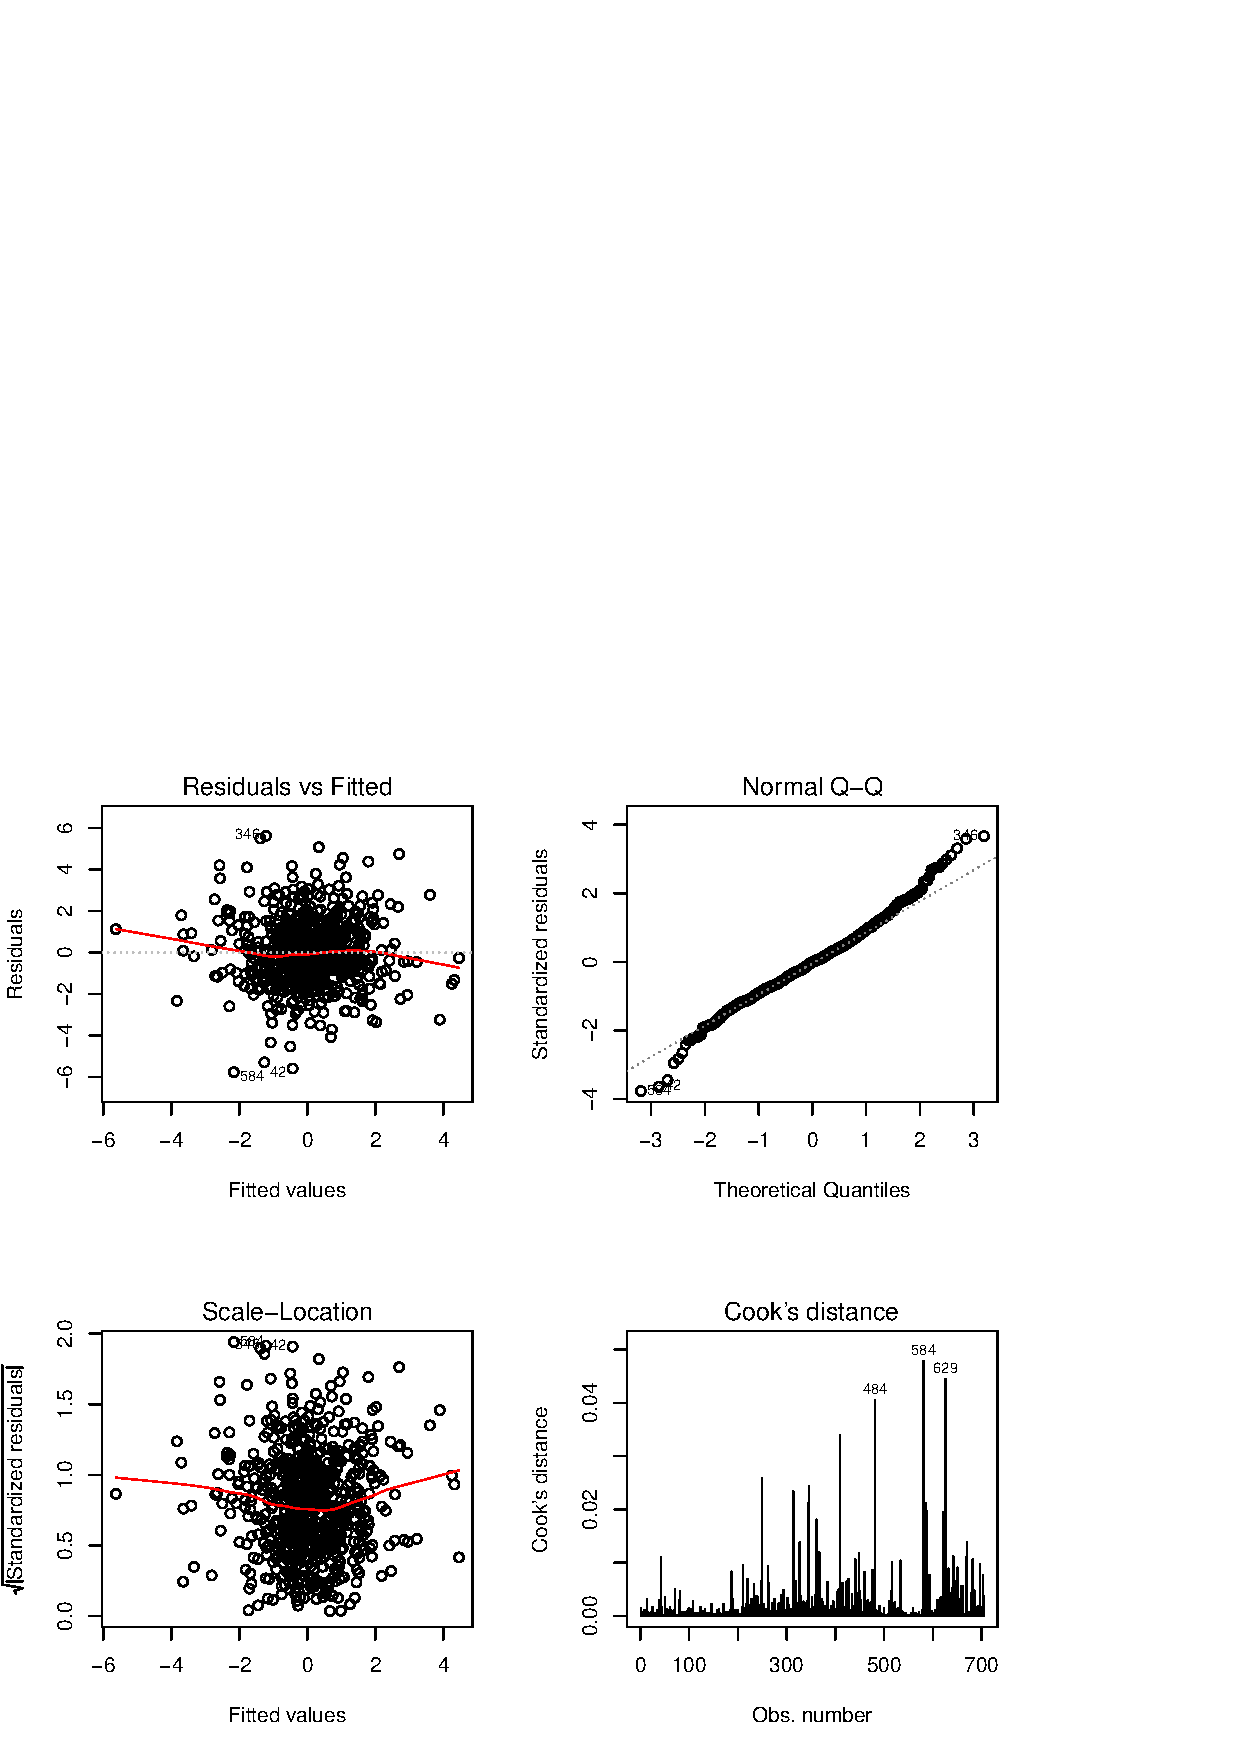
\includegraphics[width=3.3in]{fig1.pdf}
\caption{Result of GM $\sim$ Ford}
\label{fig1}
\end{figure}

Also, in Fig 1, the outputs are still not satisfactory. The residuals vs. fitted plot is not uniformly distributed, indicating the assumption that the relationship is linear may not be reasonable. Plus, there still exists some points that are far from others, implying existance of potential outliers. The normal Q-Q plot does not follow a straight line. Not all values are normally distributed. Similar to the residual plot, the scale location plot are not homogeneous neither. And the cook's distance of some points are still larger than others, which means they are not equally weighted. According to the plots, linear model is not sufficient to characterize the relationship between the log returns. 


\section{Conclusion}
Given the log return of Toyota, Ford and GM, linear regression was performed, trying to find the potential price relationship between the three auto manufactures. However, the results show their linear relations are not clear. Though the log return of GM and Ford are positively correlated, they cannot be expressed in a linear model. Some more advanced non-linear model will be tested in future works.  


% conference papers do not normally have an appendix


% use section* for acknowledgment
%\section*{Acknowledgment}


%The authors would like to thank...


% trigger a \newpage just before the given reference
% number - used to balance the columns on the last page
% adjust value as needed - may need to be readjusted if
% the document is modified later
%\IEEEtriggeratref{8}
% The "triggered" command can be changed if desired:
%\IEEEtriggercmd{\enlargethispage{-5in}}

% references section

% can use a bibliography generated by BibTeX as a .bbl file
% BibTeX documentation can be easily obtained at:
% http://mirror.ctan.org/biblio/bibtex/contrib/doc/
% The IEEEtran BibTeX style support page is at:
% http://www.michaelshell.org/tex/ieeetran/bibtex/
%\bibliographystyle{IEEEtran}
% argument is your BibTeX string definitions and bibliography database(s)
%\bibliography{IEEEabrv,../bib/paper}
%
% <OR> manually copy in the resultant .bbl file
% set second argument of \begin to the number of references
% (used to reserve space for the reference number labels box)
\begin{thebibliography}{3}

\bibitem{ref1}
Investopedia.  \emph{http://www.investopedia.com/terms/d/deadcatbounce.asp}

\bibitem{ref2}
Brian Kelly, CNN.  \emph{http://www.cnbc.com/id/102147311}

\bibitem{ref3}
Linear Regression.  \emph{https://en.wikipedia.org/wiki/Linear\_regression}

\end{thebibliography}

\newpage
\appendices

\setcounter{figure}{0}
\setcounter{table}{0}  


\section{Linear regression on the entire dataset}

\begin{table}[!h]
\centering
\caption{Result of GM $\sim$ Toyota + Ford}
\begin{tabular}{lllll}
\hline
Residuals:        &             &               &           &                       \\
\hline
Min               & 1Q          & Median        & 3Q        & Max                   \\
-6.2848           & -0.9649     & -0.0405       & 0.8977    & 5.7515                \\
\hline
\hline
Coefficients:     & Estimate    & Std. Error    & t value   & Pr($>|t|$)   \\
\hline
(Intercept)       & 0.007049     & 0.059138       & 0.119    & 0.905  \\
Toyota				   & 0.061321   & 0.037840     & 1.621     & 0.106 \\
Ford               & 0.614496     & 0.031322       & 19.619     & \textless2e-16         ***\\
\hline
\hline
\multicolumn{5}{l}{Signif. codes:  0 '***' 0.001 '**' 0.01 '*' 0.05 '.' 0.1 ' ' 1}  \\
\multicolumn{5}{l}{Residual standard error: 1.572 on 706 degrees of freedom}        \\
\multicolumn{5}{l}{Multiple R-squared:  0.3775,    Adjusted R-squared:  0.3757}     \\
\multicolumn{5}{l}{F-statistic: 214.1 on 1 and 706 DF,  p-value: \textless 2.2e-16} \\
\hline

\end{tabular}
\end{table}

\begin{figure}[!h]
\centering
\includegraphics[width=3.3in]{fig2.pdf}
\caption{Result of GM $\sim$ Toyota + Ford}
\end{figure}

\vfill
\section{R code}
\# read data \\
data.full $<-$ read.csv("E:\textbackslash\textbackslash QCF\textbackslash\textbackslash 2016Spring\textbackslash\textbackslash Finan-cialDataAnalysis\textbackslash\textbackslash hw1\textbackslash\textbackslash w\_logret\_3automanu.csv", header = FALSE) \\
data.full $<-$ data.full * 100 \\

\# summary \\
summary(data.full) \\

\# linear regression on the entire dataset \\
lm.full $<-$ lm(V3~V1+V2, data = data.full) \\
summary(lm.full) \\
par(mfrow=c(2,2))	 \\
plot(lm.full, which=c(1:4)) \\

\#remove outliers \\
data.sub $<-$ data.full[c(-311, -334, -402, -644),] \\
lm.sub $<-$ lm(V3~V1+V2, data = data.sub) \\
summary(lm.sub) \\
par(mfrow=c(2,2)) \\
plot(lm.sub, which=c(1:4)) \\

\# linear regression between GM and FORD \\
lm.ford $<-$ lm(V3$~$V2, data = data.sub) \\
summary(lm.ford) \\
par(mfrow=c(2,2)) \\
plot(lm.ford, which=c(1:4)) \\



% that's all folks
\end{document}


